% A tour of everyday Beamer, compiled by Aurora as-is.
% Build:  aurora build examples/tour/deck.tex
% PDF:    pdflatex deck && biber/bibtex … (it is ordinary Beamer)
\documentclass[aspectratio=169,xcolor=table]{beamer}
\usetheme{Madrid}
\usepackage{amsmath, amssymb}
\usepackage{booktabs, multirow}
\usepackage{listings}
\usepackage{tikz}
\usepackage{siunitx}
\usepackage{natbib}
\usepackage{aurora}

\graphicspath{{figures/}}
\lstset{language=Python, numbers=left}
\setbeamertemplate{theorems}[numbered]
\setbeamercovered{transparent}

\title[Beamer Tour]{A Tour of Everyday Beamer}
\subtitle{Overlays, structure, maths, code, figures and references}
\author[A.~Author \and B.~Author]{Ada Author\inst{1} \and Bo Author\inst{2}}
\institute{\inst{1}University of Somewhere \and \inst{2}Institute of Elsewhere}
\date[Oct 2026]{Aurora Workshop, October 2026}

\newcommand{\R}{\mathbb{R}}
\newcommand{\highlight}[1]{\textcolor{orange}{\textbf{#1}}}
\newtheorem{conjecture}[theorem]{Conjecture}
\newenvironment{keypoint}{\begin{block}{Key point}}{\end{block}}

\AtBeginSection[]{
  \begin{frame}{Outline}
    \tableofcontents[currentsection]
  \end{frame}
}

\begin{document}

\begin{frame}
  \titlepage
\end{frame}

\begin{frame}{Outline}
  \tableofcontents
\end{frame}

\section{Overlays}
\subsection{Incremental lists}

\begin{frame}[label=overlays]{Incremental lists}
  \begin{itemize}[<+-| alert@+>]
    \item First, each item appears and is highlighted while it is new
    \item Then the next one takes over
    \item Specs like \texttt{<+-| alert@+>} work on whole lists
  \end{itemize}
  \pause
  \begin{enumerate}[(a)]
    \item<5-> custom enumerate labels
    \item<6-> with explicit overlays \only<6>{(only on step 6)}
  \end{enumerate}
\end{frame}

\begin{frame}{Swapping content with \texttt{\textbackslash only} and \texttt{overprint}}
  \begin{columns}[T]
    \column{0.48\textwidth}
      \only<1>{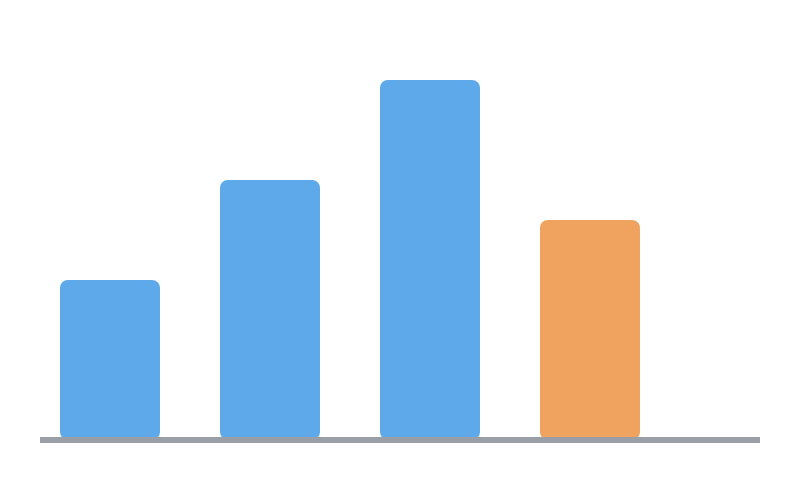
\includegraphics[width=0.9\linewidth]{bars}}
      \only<2->{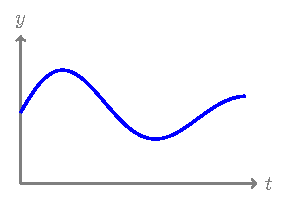
\includegraphics[width=0.9\linewidth]{diagram}}
      \centering
      \alt<1>{A bar chart (PNG)}{A damped wave (PDF)}
    \column{0.48\textwidth}
      \begin{overprint}
        \onslide<1>
          \begin{block}{Step one}
            The left figure is a PNG file.
          \end{block}
        \onslide<2>
          \begin{alertblock}{Step two}
            Now it is a PDF, rasterised at build time.
          \end{alertblock}
        \onslide<3>
          \begin{exampleblock}{Step three}
            \texttt{overprint} reserves room for its tallest part.
          \end{exampleblock}
      \end{overprint}
  \end{columns}
\end{frame}

\begin{frame}{Covered items and bare \texttt{\textbackslash onslide}}
  With \texttt{\textbackslash setbeamercovered\{transparent\}}, future content shows faintly:
  \begin{itemize}
    \item<1-> Always here
    \item<2-> From step two, \textbf<3>{bold on step three}
    \item<3-> From step three
  \end{itemize}
  \onslide<4->
  A paragraph uncovered by a bare \texttt{\textbackslash onslide<4->} switch.
\end{frame}

\begin{frame}{TikZ with overlays}
  \begin{center}
  \begin{tikzpicture}[scale=1.4]
    \draw[->] (0,0) -- (5,0) node[right] {$x$};
    \draw[->] (0,0) -- (0,3) node[above] {$f(x)$};
    \pause
    \draw[blue, very thick] (0.2,2.6) .. controls (1.5,-0.5) and (3.5,-0.5) .. (4.8,2.6);
    \pause
    \fill[orange] (2.5,0.35) circle (3pt) node[below=4pt] {$x^\ast$};
  \end{tikzpicture}
  \end{center}
\end{frame}

\section{Layout}

\begin{frame}{Columns, blocks and figures}
  \begin{columns}
    \begin{column}{0.5\textwidth}
      \begin{block}{Block}
        Standard block.
      \end{block}
      \begin{alertblock}{Alert block}
        Something important.
      \end{alertblock}
      \begin{exampleblock}{Example block}
        Something illustrative.
      \end{exampleblock}
    \end{column}
    \begin{column}{0.45\textwidth}
      \begin{figure}
        \centering
        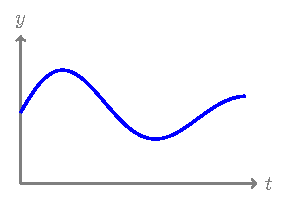
\includegraphics[width=\linewidth]{diagram}
        \caption{A PDF figure found via \texttt{\textbackslash graphicspath}.}
      \end{figure}
    \end{column}
  \end{columns}
\end{frame}

\begin{frame}{Tables}
  \centering
  \begin{tabular}{lrrr}
    \toprule
    Solver & Steps & Time (\si{\milli\second}) & Error \\
    \midrule
    Euler & 1000 & 12.1 & $1.2\times10^{-2}$ \\ \pause
    Heun  & 500  & 9.8  & $3.4\times10^{-4}$ \\ \pause
    RK4   & 100  & 4.2  & $\mathbf{2.1\times10^{-7}}$ \\
    \bottomrule
  \end{tabular}

  \bigskip
  \begin{quote}
    ``Make it work, make it right, make it fast.'' --- Kent Beck
  \end{quote}
\end{frame}

\begin{frame}{Text}
  \begin{description}
    \item[Emphasis] \emph{emph}, \textbf{bold}, \textit{italic}, \textsc{Small Caps}, \texttt{mono}, \underline{under}
    \item[Colour] \textcolor{blue}{blue}, \textcolor{red!70!black}{dark red}, \colorbox{yellow!30}{boxed}, \alert{alert}
    \item[Sizes] {\tiny tiny} {\small small} {\large large} {\Large Large}
    \item[Accents] Erd\H{o}s, Poincar\'e, G\"odel, \v{C}ech, Fran\c{c}ois, \AA ngstr\"om
    \item[Symbols] \checkmark\ \textdegree C \ldots\ \copyright\ 2026 --- en--dash
  \end{description}
\end{frame}


\section{Maths and code}
\subsection{Equations}

\begin{frame}{Numbered equations and references}
  The heat equation \eqref{eq:heat} with initial data \eqref{eq:init}:
  \begin{align}
    \partial_t u &= \kappa\, \Delta u \label{eq:heat} \\
    u(x, 0) &= u_0(x) \label{eq:init}
  \end{align}
  \pause
  Its solution on $\R^n$ is a convolution with the heat kernel:
  \begin{equation}
    u(x,t) = \int_{\R^n} \frac{e^{-|x-y|^2/4\kappa t}}{(4\pi\kappa t)^{n/2}}\, u_0(y)\,\mathrm{d}y.
  \end{equation}
\end{frame}

\begin{frame}{Overlays inside an equation}
  \[
    (a+b)^2 \only<1>{= (a+b)(a+b)}\only<2->{= a^2 + \alert<2>{2ab} + b^2}
  \]
  \uncover<3->{
    \[ \sum_{k=0}^{n} \binom{n}{k} a^{k} b^{n-k} = (a+b)^n \]
  }
  \visible<4>{The binomial theorem generalises the square: \highlight{try $n=3$}.}
\end{frame}

\subsection{Theorems}

\begin{frame}{Theorem environments}
  \begin{definition}[Prime]
    An integer $p>1$ is \emph{prime} if its only divisors are $1$ and $p$.
  \end{definition}
  \pause
  \begin{theorem}[Euclid]
    There are infinitely many primes.
  \end{theorem}
  \pause
  \begin{proof}
    Suppose $p_1,\dots,p_n$ are all of them; then $p_1\cdots p_n+1$ has a new prime factor.
  \end{proof}
  \pause
  \begin{conjecture}[Twin primes]
    There are infinitely many primes $p$ with $p+2$ prime.
  \end{conjecture}
\end{frame}

\subsection{Code}

\begin{frame}[fragile]{Listings with highlighting}
\begin{lstlisting}[caption={Newton's method}]
def newton(f, df, x, tol=1e-12):
    """Find a root of f starting from x."""
    while abs(f(x)) > tol:   # quadratic convergence
        x -= f(x) / df(x)
    return x
\end{lstlisting}
\end{frame}

\begin{frame}[fragile]{Code that builds up: \texttt{semiverbatim}}
\begin{semiverbatim}
int main(void) \{
    int n = read();
\pause
    for (int i = 0; i < n; i++)
        \alert<2>{total += i;}
\pause
    printf("%d\\n", total);
    return 0;
\}
\end{semiverbatim}
\end{frame}

\section{Wrapping up}

\begin{frame}{Units, footnotes and links}
  \begin{itemize}
    \item Speed of light: \SI{299792458}{\meter\per\second}
    \item Gravity: \qty{9.81}{\meter\per\second\squared}, Avogadro \num{6.022e23}
    \item A remark with a footnote\footnote{Footnotes collect at the bottom of the frame.}
    \item Jump back to the \hyperlink{overlays}{\beamergotobutton{overlay demo}}
  \end{itemize}
  \vfill
  \begin{keypoint}
    Everything here is plain Beamer: the same file builds a PDF with \texttt{pdflatex}.
  \end{keypoint}
\end{frame}

\begin{frame}{Related work}
  Diffusion goes back to \citet{fourier1822}; modern treatments include
  \citet{evans2010} and the numerical survey by \citet{leveque2007}.
  Kernel methods \citep[see][ch.~2]{evans2010} remain popular.
\end{frame}

\begin{frame}[allowframebreaks]{References}
  \bibliographystyle{plainnat}
  \bibliography{refs}
\end{frame}

\begin{frame}[plain,c]
  \begin{center}
    {\Huge Questions?}\\[1em]
    \url{https://github.com/aurora-slides/aurora}
  \end{center}
\end{frame}

\appendix
\begin{frame}[noframenumbering]{Backup: a table with every trick}
  \begin{tabular}{l|cc}
    \toprule
    \multirow{2}{*}{Method} & \multicolumn{2}{c}{Error} \\
                            & $L^2$ & $L^\infty$ \\
    \midrule
    \rowcolor{blue!15} Euler & $10^{-2}$ & $10^{-1}$ \\
    RK4 & $10^{-6}$ & \cellcolor{teal!25}$10^{-5}$ \\
    \bottomrule
  \end{tabular}
\end{frame}

\end{document}
